This section gives the explanation of architectural pattern and more detailed implementation of the server side. 

% Architecture MV, , JWT for Auth, Websocket Dispatcher, Resource Listening?

\subsection{Architecture}

\subsubsection{MVC Pattern and Project Structure}
To separate the different layers of model, view and controller, \gls{MVC} pattern is used as the basic pattern of the architecture. In the model layer, all data model related concerns such as data shema definitions, data model validation as well as database operations are defined. And Controllers contain the core domain logics, process the data from model layer, and pass the result to view layer.

Since the templates are rendered on the client side, the view layer is just simply stripped. Therefore, basically the controllers response processed data to client side directly without rendering it to views. Figure \ref{fig:server-file-structure-imp} shows the overview of the server's  file structure which is featured with MVC pattern.

\begin{figure}[!htbp]
\centering
\begin{forest}
  for tree={
    font=\ttfamily,
    grow'=0,
    child anchor=west,
    parent anchor=south,
    anchor=west,
    calign=first,
    edge path={
      \noexpand\path [draw, \forestoption{edge}]
      (!u.south west) +(7.5pt,0) |- node[fill,inner sep=1.25pt] {} (.child anchor)\forestoption{edge label};
    },
    before typesetting nodes={
      if n=1
        {insert before={[,phantom]}}
        {}
    },
    fit=band,
    before computing xy={l=15pt},
  }
[server
  [config/
    [index.js]
    [routes.js]
  ]
  [models/]
  [controllers/]
  [index.js]
  [...]
]
\end{forest}
\caption{Overview of server app's file structure}
\label{fig:server-file-structure-imp}
\end{figure}


\begin{enumerate}
\item 
  \textbf{index.js}: the entry point of the whole server app. It will create a server instance and set up configurations for the server. In addition, a connection from server instance to database will be established. After all configurations are done, the server instance will start listening port and waiting for the requests from client.
\item
  \textbf{config/index.js}: config as well as constants for the server. It persists \textit{apiConfig} for example the common prefix of API URL and version of the API. And config for database including the database URL will be defined here as well. In addition, keys for encryption are also stored in the config file.
\item
  \textbf{config/routes.js}: rules for URL matching. All URL matching rules are defined in this file. Controllers are referenced here and a dispatcher for router will be instantiated. If any request meets the defined rule, the request will be forward to a correlative controller. 
\item
  \textbf{controllers/*}: controllers for processing specific requests.
\item 
  \textbf{models/*}: data model definitions. Files under this directory are organized by different data domain.
\end{enumerate}


\subsubsection{Achitecture of Server}

The figure \ref{fig:server-arch-imp} illustrates an overview of the server's architecture. 

\begin{figure}[!htbp]
  \centering
    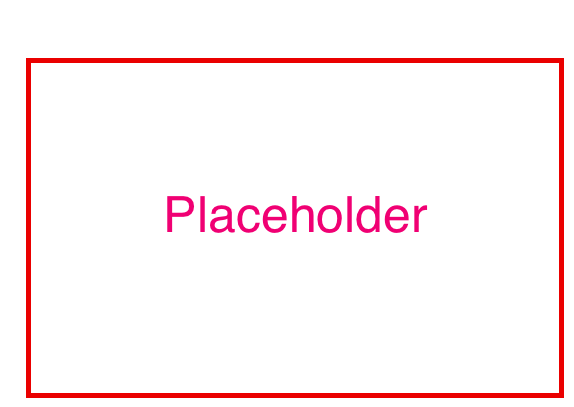
\includegraphics[width=0.6\textwidth]{Figures/placeholder.png}
  \caption{placeholder}
  \label{fig:server-arch-imp}
\end{figure}
% process of request to be handeled. index.js -> create server isntance -> connect to database. routes -> different controllers -> different models

\subsection{Data Schema Definition}